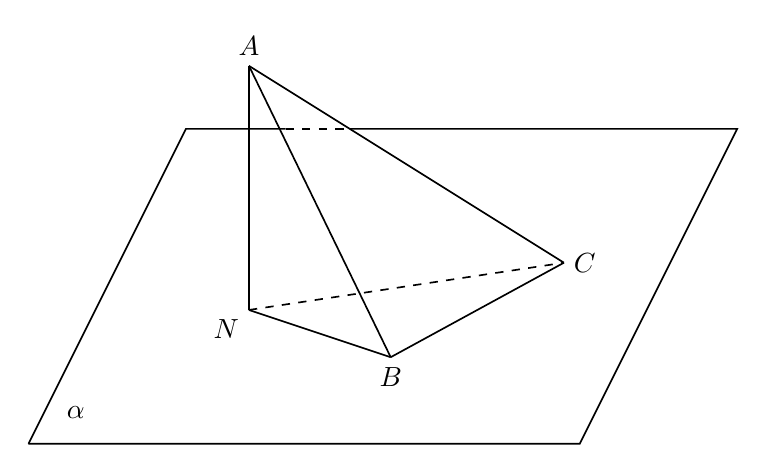
\begin{tikzpicture}[line width=.6pt, font=\normalsize]
  % plane alpha as parallelogram
  \coordinate (P1) at (-4,-2);
  \coordinate (P2) at (3,-2);
  \coordinate (P3) at (5,2);
  \coordinate (P4) at (-2,2);
  \draw (P1) -- (P2) -- (P3) -- (0.08,2);
  \draw (P1) -- (P4) -- (-0.735483871,2);
  \draw[dashed] (-0.735483871,2) -- (0.08,2);
  % tetrahedron N-ABC, A above plane, N,B,C on plane
  \coordinate (N) at (-1.2,-0.3);
  \coordinate (A) at (-1.2,2.8);
  \coordinate (B) at (0.6,-0.9);
  \coordinate (C) at (2.8,0.3);
  \draw (A) -- (N);
  \draw (A) -- (B);
  \draw (A) -- (C);
  \draw (N) -- (B);
  \draw (B) -- (C);
  \draw[dashed] (N) -- (C);
  \node[above] at (A) {$A$};
  \node[below left] at (N) {$N$};
  \node[below] at (B) {$B$};
  \node[right] at (C) {$C$};
  \node at (-3.4,-1.6) {$\alpha$};
\end{tikzpicture}
